\chapter{Methodology}

This chapter describes the methodological framework used to examine the effects of an AI-guided virtual-reality (VR) meditation system on users’ stress, mindfulness, affect, workload, and overall experience.  
It outlines the research design, participant characteristics, hardware and software setup, experimental procedure, measurement instruments, data collection and processing steps, statistical analyses, and ethical considerations.

\section{Research Design}
The primary aim of this study was to compare the effectiveness of two meditation modalities in reducing stress after a common stress induction: 
(a) conventional meditation and 
(b) AI-guided virtual reality (VR) meditation.

A mixed experimental design was adopted, combining:
\begin{itemize}
    \item a \textbf{between-subjects factor}: meditation modality (conventional vs.\ AI-guided VR), and
    \item a \textbf{within-subjects factor}: experimental phase (stress induction, meditation).
\end{itemize}

All participants first completed a resting \emph{baseline} phase, followed by a \emph{stress-induction} phase using the game \emph{Flappy Bird}, and then a \emph{meditation} phase. 

The Flappy Bird task was used to elevate arousal and induce a comparable stress level across participants before the relaxation intervention. Participants were then randomly assigned to either the conventional meditation condition or the AI-guided VR meditation condition, where stress recovery was expected to occur.

Physiological signals (heart rate, heart-rate variability, skin conductance, skin temperature, pulse volume amplitude, and motion amplitude) were recorded continuously across all phases using the Biofeedback 2000 Xpert system. Stress reduction was operationalized as the change in physiological indices from the stress phase to the meditation phase (e.g., a decrease in SCL and heart rate, and an increase in HRV). These changes were compared between the two meditation groups to determine which modality produced stronger recovery from the induced stress. Physiological signals were recorded for offline analysis only and were not used to adapt the VR environment or the AI guidance in real time.


Self-report questionnaires were collected only after the meditation phase; therefore, subjective outcomes follow a between-subjects comparison only, while physiological responses support both within-subject (phase-based) and between-subject (modality-based) analyses.

\section{Experimental Setup}
\subsection{Rationale for Using Virtual Reality Instead of 2D Displays}

A central design decision in this study was the use of a fully immersive Virtual Reality (VR) environment rather than a conventional 2D display such as a television, monitor, or mobile device. This choice is grounded in both theoretical and empirical evidence on how immersion, attentional focus, and sensory isolation influence the quality of meditation and emotional regulation.

VR offers the advantage of \textbf{high presence}, defined as the subjective feeling of “being there” which is strongly associated with deeper engagement and reduced susceptibility to external distractions \cite{slater2018immersive,jerald2016vrbook}. In contrast, 2D displays allow continuous exposure to the surrounding environment, ambient noise, and visual disturbances, which can interfere with meditative focus.

Furthermore, immersive VR environments provide \textbf{full-field visual occupation} and spatial audio, creating a controlled sensory envelope ideal for guiding relaxation and regulating breathing. Prior research demonstrates that VR meditation enhances emotion regulation, reduces anxiety, and improves attentional stability more effectively than non-immersive media \cite{tarrant2018virtual,liszio2018nature}. 

For the AI-guided component, VR also enables \textbf{embodied interaction}—the user perceives AI-guided voice prompts as originating from within the virtual space, creating stronger perceived connectedness and therapeutic engagement compared to listening through a TV or phone speaker.  

Table~\ref{tab:vr-vs-2d} summarizes the key differences between VR-based meditation and conventional 2D meditation environments with respect to immersion, attentional focus, and environmental control. Given these benefits, VR was selected to maximize immersion, minimize distraction, and create an optimally controlled environment for studying stress-reduction and physiological regulation.


\begin{table}[H]
\centering
\caption{Conceptual comparison of VR-based versus 2D-based meditation delivery, based on immersion theory and prior VR meditation literature \cite{slater2018immersive,jerald2016vrbook,tarrant2018virtual,liszio2018nature}
}
\label{tab:vr-vs-2d}
\begin{tabular}{p{4cm} p{5cm} p{5cm}}
\hline
\textbf{Feature} &
\textbf{VR Meditation (HTC Vive Pro)} &
\textbf{2D Meditation (TV/Laptop)} \\
\hline
Immersion &
High immersion via stereoscopic 3D, spatial audio, and presence &
Low immersion; flat screen with no spatial congruence \\
\hline
Distraction Level &
Reduced external visual distraction (sensory occlusion by HMD) &
External environment remains visible; distraction depends on setting \\
\hline
Environmental Control &
Complete simulated environment &
Environment cannot be controlled \\
\hline
Emotional Engagement &
Often reported as higher immersion &
Lower immersion; engagement depends on content \\
\hline
Attentional Focus &
Often higher due to presence/occlusion (reported in prior work) &
More susceptible to external cues \\
\hline
Suitability for Adaptive cues &
Highly suitable for embodied/immersive cues &
Possible but less embodied\\
\hline
Meditation Depth &
May support perceived deeper engagement via immersion &
Engagement depends on the setting and the user \\
\hline
\end{tabular}
\end{table}

The comparison in Table~\ref{tab:vr-vs-2d} is intended as a conceptual rationale rather than an empirical result.
It is grounded in presence and immersion theory \cite{slater2018immersive,jerald2016vrbook} and supported by prior studies reporting beneficial effects of VR meditation on affect and attentional engagement \cite{tarrant2018virtual,liszio2018nature}.
Furthermore, VR environments support adaptive scene transitions (e.g., breathing visuals) that align dynamically with AI-guided instructions. Such adaptive cues are less perceptually impactful when delivered on a standard screen. For these reasons, VR is the most suitable medium for delivering a controlled, immersive, and emotionally effective meditation experience.


\subsection{Hardware Materials}
The VR condition was presented using an \textbf{HTC Vive Pro} head-mounted display.
Physiological signals were recorded with the \textbf{Biofeedback 2000 Xpert} system (Schuhfried GmbH).
All sessions were run on a dedicated workstation to ensure stable VR rendering and reliable data logging.


\subsubsection{HTC Vive Pro Head-Mounted Display}
The experiment used an \textbf{HTC Vive Pro} HMD providing stereoscopic VR with a combined resolution of
2880$\times$1600 pixels, a 90\,Hz refresh rate, and an approximately 110$^\circ$ field of view \cite{htc_vive_pro}.
The headset was operated via SteamVR and connected to the Unity-based application used in this study.
No eye tracking was used (standard Vive Pro configuration).


\begin{figure}[H]
    \centering
    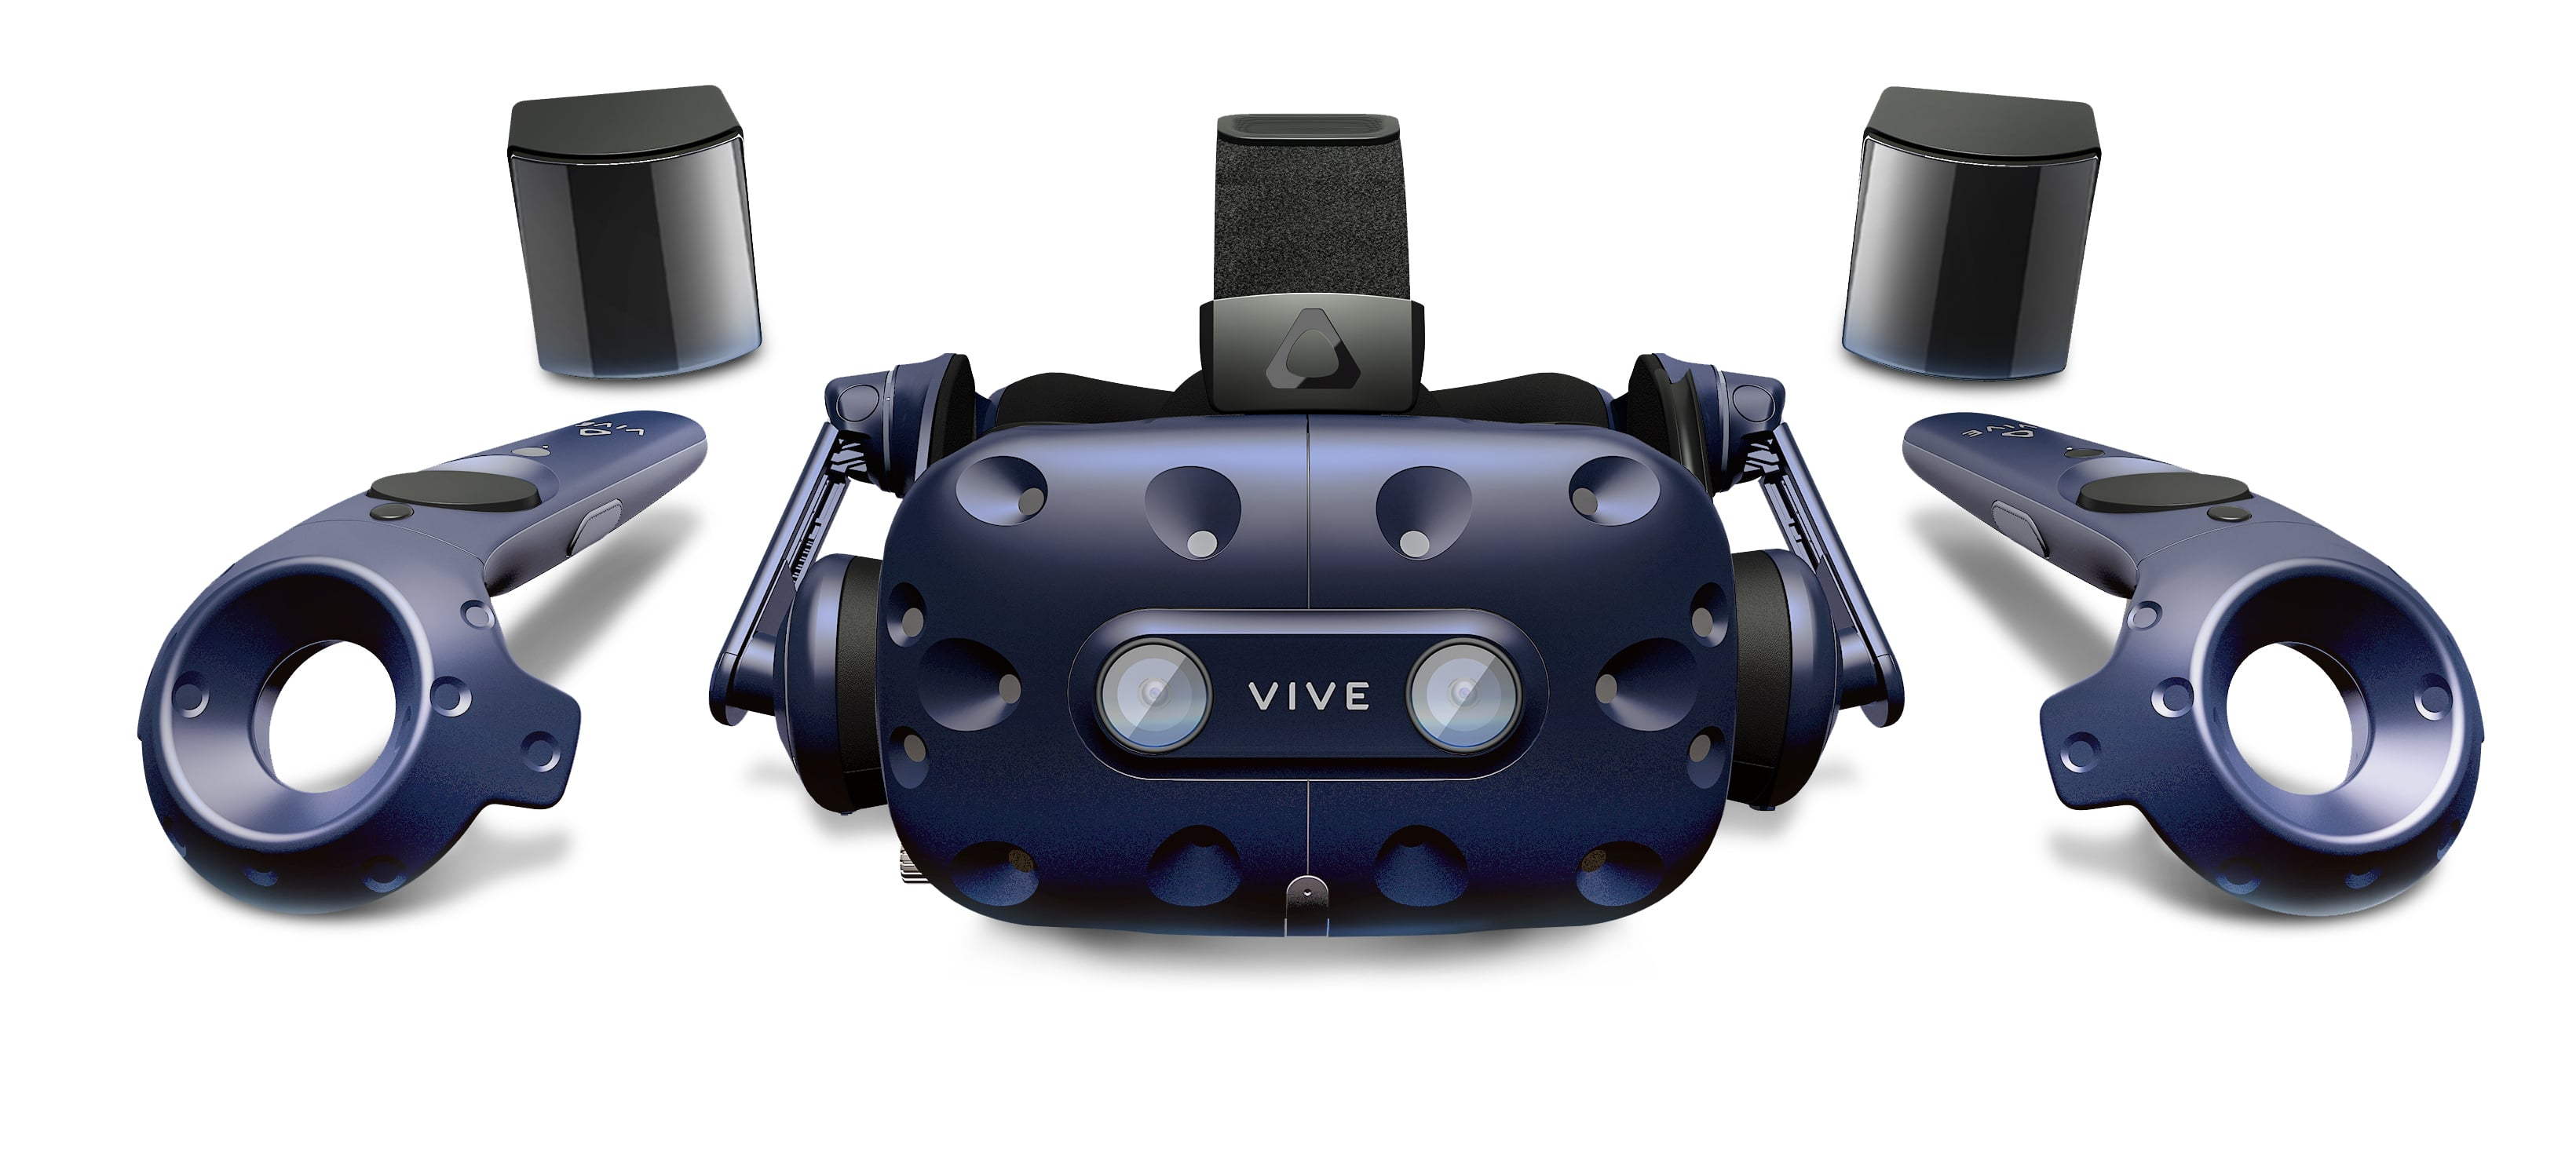
\includegraphics[width=0.60\textwidth]{pics/20180424-tw-news-min.jpg}
    \caption{HTC VIVE Pro head-mounted display\cite{htc_vive_pro}.}
    \label{fig:HTC_Vive_pro}
\end{figure}



\subsubsection{Biofeedback 2000 Xpert System}
\label{sec:biofeedback}
Physiological data were recorded using the \textbf{Biofeedback 2000 Xpert} system \cite{schuhfried_biofeedback2000xpert}.
The following signals were acquired: \textit{blood volume pulse (BVP)} for heart rate and HRV,
\textit{electrodermal activity (SCL/SCR)}, and \textit{skin temperature}. Data were stored for offline analysis. Further details on sensor placement, acquisition settings, preprocessing, and feature extraction are provided in Appendix~\ref{app:physio}.


\begin{figure}[H]
    \centering
    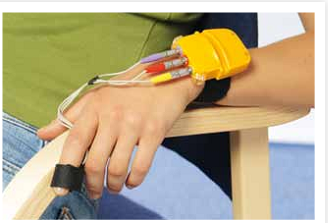
\includegraphics[width=0.60\textwidth]{pics/biofeedback-xpert_device.png}
    \caption{Biofeedback 2000 Xpert system used for physiological recording \cite{schuhfried_biofeedback2000xpert}.}
    \label{fig:bio-xpert}
\end{figure}

\paragraph{Workstation}

All VR sessions and data processing were performed on a high-performance workstation
with the following specifications shown in table~\ref{tab:workstation}:

\begin{table}[H]
\centering

\caption{Workstation configuration used for VR rendering and data analysis.}
\label{tab:workstation}
\begin{tabular}{ll}
\toprule
\textbf{Component} & \textbf{Specification} \\
\midrule
CPU & Intel Core i9-11900K (3.50\,GHz) \\
RAM & 128\,GB DDR4 \\
GPU & NVIDIA GeForce RTX 3090 Ti (24\,GB) \\
Storage & 16.4\,TB (SSD + HDD) \\
System & Windows 11, 64-bit \\
\bottomrule
\end{tabular}

\end{table}


\subsection{Software and Environment}
The implementation of the VR meditation system and the overall experimental workflow required several software components working together across content creation, artificial intelligence processing, physiological signal acquisition, and data analysis. The following subsections describe the main software tools and frameworks used in this study.

\subsubsection{Unity Engine}

The virtual environment and meditation application were developed using the \textbf{Unity} game engine (Version 2021.x). Unity was selected due to its stability, extensive VR support, and ability to integrate custom interaction logic, AI-driven components, and external hardware. The application includes the VR scene, audio pipeline, visual transitions (light fading, skybox changes), and user interaction logic. Unity’s coroutine system and animation curves were used to implement smooth temporal effects such as visual changes.

\subsubsection{SteamVR / OpenXR Runtime}

VR rendering and headset tracking were enabled using the \textbf{SteamVR} framework with the \textbf{OpenXR} backend, which ensured compatibility with the HTC Vive Pro headset. SteamVR manages:
\begin{itemize}
    \item stereoscopic rendering,
    \item Lighthouse positional tracking,
    \item headset orientation updates,
    \item frame-timing and reprojection.
\end{itemize}

This ensures low-latency head tracking and stable frame rates, both critical for immersion and preventing cybersickness during meditation.

\subsubsection{OpenAI GPT and Text-to-Speech Integration}

Meditation guidance in the VR condition was generated dynamically during the session in real time using the OpenAI
GPT language model, accessed via the official Chat Completions API
\cite{openai_gpt}. During the session, the Unity application sent short cue prompts
together with the participant's reported stress level to GPT and received concise, calming guidance
sentences in return.

These sentences were immediately forwarded to an online Google Text-to-Speech (TTS)
service, which converted the text into audio. The resulting audio streams were
played back inside the VR scene through Unity's \texttt{AudioSource} component,
providing a continuous sequence of adaptive, AI-generated meditation prompts. A
more detailed description of this pipeline is provided in
Section~\ref{sec:ai-meditation-pipeline}.


\subsubsection{Biofeedback 2000 Xpert Software}

Physiological signals were recorded using the \textbf{Biofeedback 2000 Xpert} software suite, which supports real-time acquisition of:
\begin{itemize}
    \item Blood Volume Pulse (BVP),
    \item Skin Conductance Level (SCL),
    \item Skin Temperature (TEMP),
    \item Pulse Volume Amplitude (PVA),
    \item Pulse Frequency.
\end{itemize}

The software automatically time-stamps all signals and logs them to .xls for offline analysis. Session markers corresponding to the experimental phases (baseline, stress induction, meditation) were inserted manually during data collection.

\subsubsection{Python for Data Processing}

Post-experiment physiological data processing was conducted in \textbf{Python} using the following libraries:
\begin{itemize}
    \item \texttt{pandas} — preprocessing and time alignment,
    \item \texttt{numpy} — numerical operations,
    \item \texttt{neurokit2} — HRV extraction (RMSSD, IBI, peak detection),
    \item \texttt{matplotlib/seaborn} — visualization,
    \item \texttt{scipy} — statistical tests.
\end{itemize}

Python enabled efficient extraction of features such as HR, HRV (RMSSD), SCL means, SCR peaks, and temperature changes.

\subsubsection{Survey Platform and Statistical Tools}
Questionnaires were administered using Unipark (TIVIAN). All preprocessing, scoring, visualization, and inferential statistical analyses were performed in Python using SciPy and related libraries.


\subsubsection{Operating System and Runtime Environment}

All VR experiences were executed on a Windows 11 machine running the SteamVR runtime. Physiological recordings were performed on the Biofeedback 2000 Xpert software.

\section{AI-Guided Voice Meditation Pipeline}
\label{sec:ai-meditation-pipeline}
The AI-guided meditation in the VR condition is implemented as a pipeline consisting of three main components: (1) text generation using a large language model (GPT), (2) text-to-speech (TTS) synthesis, and (3) audio scheduling and playback in the Unity-based VR environment. No physiological measurements were used as input to the GPT model or the VR environment during the session; biofeedback data were analysed only after data collection.


\subsubsection{Meditation Script Generation via OpenAI GPT}

Meditation guidance was generated online using the \textbf{OpenAI GPT} language model (gpt-3.5-turbo) accessed via the official OpenAI Chat Completions API \cite{openai_gpt}. 
Rather than playing a fixed, pre-recorded script, the system queried GPT at runtime and received short, adaptive guidance sentences that were then converted to speech.

At the beginning of the VR session (Scene~1), a voice interaction sequence was used to initialise the system. 
The TTS component first asked the participant: \emph{``Before we start, how is your stress level: high or low?''}. 
The spoken answer was captured via a \texttt{VoiceCommandListener} and forwarded to the \texttt{OpenAIManager}, which parsed the response and stored it as an internal \texttt{StressLevel} enum (\texttt{Low}, \texttt{High}). 
This stress level was later embedded into the system prompt sent to GPT, so that all subsequent guidance could be tailored accordingly (e.g.\ slower pace for ``Low'' stress and more reassurance for ``High'' stress).

The main meditation then took place in Scene~2, controlled by a \texttt{Scene2Controller} coroutine. 
Here, the current stress level determined a binary mode (\emph{high} vs.\ \emph{low} stress), which in turn controlled the overall session duration (4~minutes for both modes) and the time gap between prompts (shorter gaps for higher stress, longer gaps for lower stress). 
The meditation flow was modelled for simple meditation cues, but instead of playing these fixed strings, each cue was sent as a user message to GPT, together with a system message such as:

\begin{quote}
``You are a meditation guide. Replies must always be under 15 words, consisting of one short, calming sentence, varied each time. The user's current stress is: [High/Low].''
\end{quote}

The \texttt{OpenAIManager} constructed the JSON payload with this system instruction and the current cue text, sent it to the OpenAI API, and parsed the returned chat response. 
From each reply, the first choice's \texttt{message.content} was extracted as a short, GPT-generated guidance sentence. 
This sentence was then passed to the TTS component, which spoke it aloud and signalled completion back to the coroutine via the \texttt{onResponseComplete} callback. 
The coroutine waited until TTS playback finished, then observed the configured silence interval (depending on stress level), and finally requested the next GPT line, continuing this cycle until the 4-minute meditation window elapsed.

In this way, the spoken meditation guidance was not a single static script but a sequence of dynamically generated, stress-sensitive micro-prompts produced by GPT in real time, while still following a deterministic temporal structure (intro, repeated inhale/exhale cues, outro) encoded in the Unity scene logic.

\subsubsection{Text-to-Speech (TTS) Synthesis}

Spoken guidance was produced using the \textbf{Google TTS} service. The selected meditation script is converted to speech with:
\begin{itemize}
    \item a neutral, calm voice profile,
    \item a slightly reduced speaking rate to support relaxation,
\end{itemize}


\subsubsection{Audio Scheduling and Playback in Unity}

Within Unity, an \texttt{AudioManager} component manages the sequencing of voice prompts. The meditation session is modeled as a simple state machine (e.g., \emph{Intro} $\rightarrow$ \emph{Main Meditation} $\rightarrow$ \emph{Closing}). When the participant’s stress level has been selected, the corresponding sequence of audio clips is loaded, and each segment is scheduled with predefined intervals.

The \texttt{AudioSource} component attached to the VR camera rig is used to render the TTS audio in spatialized form. This makes the guidance feel as though it originates from within the virtual environment rather than from an external device, supporting immersion and presence.
% \begin{figure}[H]
% \centering
% \begin{tikzpicture}[
%     node distance=1.2cm,
%     box/.style={rectangle,rounded corners,draw=black,thick,align=center,text width=3.2cm,minimum height=1.0cm},
%     arrow/.style={->, thick}
% ]

% \node[box] (stress) {Stress Input \\ (High / Low)};
% \node[box, below=of stress] (gpt) {GPT Script Selection};
% \node[box, below=of gpt] (tts) {Google TTS \\ (Audio Generation)};
% \node[box, below=of tts] (unity) {Unity Playback \\ (Audio Manager)};
% \node[box, below=of unity] (vive) {HTC Vive Pro \\ Output};

% \draw[arrow] (stress) -- (gpt);
% \draw[arrow] (gpt) -- (tts);
% \draw[arrow] (tts) -- (unity);
% \draw[arrow] (unity) -- (vive);

% \end{tikzpicture}
% \caption{Vertical AI–TTS pipeline integrating OpenAI GPT script generation and Google TTS audio synthesis.}
% 
% \end{figure}

\begin{figure}[H]
\centering
\begin{tikzpicture}[
    node distance=1.15cm,
    box/.style={
        rectangle, rounded corners,
        draw=black, thick,
        align=center,
        text width=4.4cm,
        minimum height=1.0cm
    },
    smallbox/.style={
        rectangle, rounded corners,
        draw=black, thick,
        align=center,
        text width=4.4cm,
        minimum height=0.9cm
    },
    arrow/.style={->, thick},
    dashedarrow/.style={->, thick, dashed}
]

% -----------------------
% Main vertical pipeline
% -----------------------
\node[box] (user) {User-selected stress level \\ \textbf{(High / Low)}};
\node[box, below=of user] (prompt) {Prompt / script selection \\ (condition-specific cues)};
\node[box, below=of prompt] (gpt) {OpenAI GPT \\ cue text generation};
\node[box, below=of gpt] (tts) {Google TTS \\ audio synthesis};
\node[box, below=of tts] (unity) {Unity Audio Manager \\ playback + timing control};
\node[box, below=of unity] (vr) {HTC Vive Pro \\ audio output in VR};

\draw[arrow] (user) -- (prompt);
\draw[arrow] (prompt) -- (gpt);
\draw[arrow] (gpt) -- (tts);
\draw[arrow] (tts) -- (unity);
\draw[arrow] (unity) -- (vr);

% -----------------------
% Parallel data logging (no feedback)
% -----------------------
\node[smallbox, right=2.75cm of unity] (bio) {Biofeedback sensors \\ (data logging only)};
\node[smallbox, below=of bio] (store) {Recorded dataset \\ (offline analysis)};

\draw[dashedarrow] (unity.east) -- node[above, align=center]{} (bio.west);
\draw[arrow] (bio) -- (store);

% % Optional note for clarity
% \node[align=center, font=\footnotesize, right=2.2cm of gpt] (note) {No real-time\\biofeedback loop};

\end{tikzpicture}
\caption{VR meditation audio pipeline driven by user-selected stress level. Biofeedback sensors were used for data logging and offline analysis only (no real-time feedback to GPT or VR).}
\label{fig:ai-tts-pipeline}
\end{figure}

\section{Breathing-Responsive Light and Skybox Adaptation}
\label{sec:breathing-light}

To support paced breathing during meditation, the VR environment incorporates a
dynamic ambient-light system that is synchronised with the AI-generated voice guidance.
Because participants meditate with their eyes gently closed, the skybox is configured
with a high-intensity solid colour, creating a soft diffused glow that remains
perceptible through the eyelids. This glow serves as a non-visual pacing cue: the
perceived brightness increases during inhalation and gradually decreases during
exhalation, guiding the breathing rhythm without requiring visual fixation.

Figure~\ref{fig:breathing-light} illustrates the high-intensity breathing light
used during the meditation phase.


% \begin{figure}[H]
%     \centering
%     \begin{subfigure}[b]{0.47\textwidth}
%         \centering
%         
\includegraphics[width=\textwidth]{pics/Capture 2.PNG}
%         \caption{Dimmed skybox state ("breath out"). The skybox decreases in intensity during exhalation, reinforcing slow relaxation breathing. }
%         \label{fig:skybox-inhale}
%     \end{subfigure}
%     \hfill
%     \begin{subfigure}[b]{0.47\textwidth}
%         \centering
%         
\includegraphics[width=\textwidth]{pics/3.PNG}
%         \caption{Bright skybox state ("breath in"). The solid-colour skybox increases in intensity, creating a gentle glow perceived through closed eyelids.}
%         \label{fig:skybox-exhale}
%     \end{subfigure}

%     \caption{Breathing-responsive skybox illumination. The VR environment alternates smoothly between a brighter (inhale) and darker (exhale) skybox colour, synchronised with AI-guided meditation cues.}
%     \label{fig:breathing-light}
% \end{figure}
\begin{figure}[H]
    \centering
    \begin{subfigure}[b]{0.47\textwidth}
        \centering
        
\includegraphics[height=4cm,keepaspectratio]{pics/Capture 2.PNG}
        \caption{Dimmed skybox ("breath out"). The skybox decreases in intensity during exhalation.}
        \label{fig:skybox-exhale}
    \end{subfigure}
    \hfill
    \begin{subfigure}[b]{0.47\textwidth}
        \centering
        
\includegraphics[height=4cm,keepaspectratio]{pics/3.PNG}
        \caption{Bright skybox ("breath in"). The skybox increases in intensity during inhalation.}
        \label{fig:skybox-inhale}
    \end{subfigure}
    \caption{Breathing-responsive skybox illumination synchronized with AI-guided cues.}
    \label{fig:breathing-light}
\end{figure}

The skybox behavior is governed by an \texttt{EnvironmentController} script, which animates several shader
parameters over the session:

\begin{itemize}
    \item global skybox exposure,
    \item blend transitions between ``inhale'' and ``exhale'' color schemes.
\end{itemize}

These parameters are interpolated using animation curves aligned with the
meditation timeline (introduction, breathing guidance, closing phase). Initially,
the skybox appears brighter with neutral tones; as the session progresses,
colours shift toward lower-saturation gradients, reflecting the intended transition
from alertness to calm introspection.

An example of the aurora-inspired skybox used during the meditation phase is shown in
Figure~\ref{fig:skybox-inhale} and Figure~\ref{fig:skybox-exhale}.


\subsection{Multimodal Synchronisation}

By coupling AI-guided audio, breathing-responsive illumination, and an
emissive skybox, the system delivers a coherent multimodal cueing mechanism.
Even when the eyes are closed, participants perceive a gentle pulsation of
light aligned with the breathing guidance, reducing cognitive load and
supporting stable attentional focus. The multimodal integration is designed to:

\begin{itemize}
    \item promote consistent breathing tempo,
    \item reduce visual demand compared to object-focused VR meditation,
    \item minimise mind-wandering through continuous but unobtrusive sensory input,
    \item enhance subjective depth of the meditative state.
\end{itemize}

Participant feedback (Section~\ref{sec:questionnaire_results}) indicates that most
users found the through-eyelid glow calming, whereas a minority reported
brightness sensitivity, suggesting a need for adaptive luminance control in
future versions.

\begin{figure}[H]
\centering
\begin{tikzpicture}[
    node distance=1.2cm,
    box/.style={rectangle,rounded corners,draw=black,thick,align=center,text width=4.0cm,minimum height=1.0cm},
    arrow/.style={->, thick}
]

\node[box] (audio) {AI/TTS Meditation Audio \\ (\texttt{AudioSource})};
\node[box, below=of audio] (lightScript) {\texttt{LightOnAudio} \\ (Monitor playback, fading)};
\node[box, below=of lightScript] (skybox) {Skybox Emission \\ Brightness / Exposure};
\node[box, below=of skybox, text width=5cm] (user) {Participant Perception \\ (Through-eyelid glow, breathing pacing)};

\draw[arrow] (audio) -- (lightScript);
\draw[arrow] (lightScript) -- (skybox);
\draw[arrow] (skybox) -- (user);

\end{tikzpicture}
\caption{Pipeline linking AI/TTS audio playback to skybox brightness modulation via \texttt{LightOnAudio}, producing a through-eyelid glow that supports paced breathing.}
\label{fig:light-skybox-pipeline}
\end{figure}




\subsection{Integration with Physiological Recording}
During each session, the Unity VR application and the Biofeedback~2000 Xpert system ran in parallel. Physiological signals were recorded continuously during phase boundaries (stress induction, meditation) in the Biofeedback software. The recorded time series were exported and segmented offline using these phase markers. Importantly, physiological recordings were used for data logging and offline analysis only and did not provide real-time feedback to the VR application or the GPT/TTS pipeline.


\section{Participants}

\subsection{Recruitment}
The recruitment targeted adults within the university community, without requiring prior experience in meditation or virtual reality. Participation was voluntary and uncompensated.

\subsection{Sample Characteristics}
A total of \textbf{44 participants} (7 female, 37 male) participated in the study, with an intended allocation of (23 participants in VR group and 21 participants in conventional). Participants ranged in age from 22 to 35 years and included university students and staff. Basic demographic information (meditation experience, VR familiarity) was collected through a post-session questionnaire.

\subsection{Participant Background Characteristics}

Participants reported their prior experience with meditation on a
five-point ordinal scale ranging from \textit{no experience} to
\textit{extensive experience}. This measure was included to
characterize the sample and to assess whether the two experimental
groups differed in their familiarity with meditation prior to the
study.

Descriptively, participants in the conventional meditation condition
reported higher levels of prior meditation experience than those in the
VR condition (Table~\ref{tab:meditation-experience}). In the conventional
group, 8 out of 21 participants (approximately 38.09\%) indicated regular
or extensive experience with meditation. In contrast, the VR group
contained a higher proportion of meditation-naive participants. with
9 out of 23 participants (approximately 39.13\%) who did not have prior
meditation experience.

Both groups nonetheless included a mix of experience levels, and no
formal inferential statistical test was applied, as this variable was
intended for descriptive sample characterization rather than hypothesis
testing.

\begin{table}[H]
\centering
\caption{Distribution of prior meditation experience by meditation method.}
\label{tab:meditation-experience}
\begin{tabular}{lccccc}
\toprule
\textbf{Method} & \textbf{No experience} & \textbf{Very little} & \textbf{Some} & \textbf{Regular} & \textbf{Extensive} \\
\midrule
Conventional & 4 & 6 & 3 & 5 & 3 \\
VR           & 9 & 6 & 4 & 3 & 1 \\
\bottomrule
\end{tabular}
\end{table}



\subsection{Inclusion Criteria}
Participants were eligible if they met the following criteria:
\begin{itemize}
    \item Age 18 years or older
    \item Normal or corrected-to-normal vision
    \item Willingness to wear physiological sensors (Biofeedback 2000 Xpert)
    \item No known medical contraindications for VR use
\end{itemize}

\subsection{Exclusion Criteria}
Participants were excluded based on any of the following conditions:
\begin{itemize}
    \item History of epilepsy or photosensitive seizures
    \item Severe susceptibility to motion sickness
    \item Cardiovascular abnormalities that interfere with physiological measurement (e.g., arrhythmia)
    \item Skin allergies to adhesive electrodes used for SCL/BVP recording
    \item Current treatment for severe anxiety, PTSD, or other conditions that may interact with meditation tasks
    \item Prior participation in a similar VR meditation pilot test
\end{itemize}

\subsection{Sample Size Justification}
An a priori power analysis was performed using G*Power 3.1 \cite{Faul2007GPower3} for an independent-samples t-test with medium effect size (Cohen's $d = 0.5$), a two-tailed test, and a significance level of $\alpha = 0.05$. The analysis indicated that achieving 80\% power would require a total of $N = 128$ participants (64 per group). 

Recruiting the statistically ideal sample size was not feasible due to the logistical constraints of VR-based physiological recordings, including session duration and sensor setup. Similar VR-based psychophysiology studies typically include 20–45 participants (typical for VR psychophysiology) \cite{weibel2020biofeedback,brief2025vrbiofeedback, Zimmer2019VR_TSST,rodrigues2021IMVEST}. 

Accordingly, the present study targeted a realistic sample size of approximately 40-50 participants and ultimately recruited $N = 44$ participants. A post-hoc power estimate for this sample size produced an achieved statistical power of approximately $0.36$ (see Figure~\ref{fig:gpower44}), which is acceptable for an exploratory or pilot study designed to detect medium and larger effects. Figure~\ref{fig:powercurve} illustrates how statistical power increases with total sample size for a medium effect ($d = 0.5$). At the actual sample of $N = 44$, the achievable power is approximately $0.36$, which is typical for exploratory or pilot studies of this scope.


\begin{figure}[H]
    \centering
    
\includegraphics[width=0.85\textwidth]{graphs/power graph.png}
    \caption{G*Power X–Y plot illustrating the required total sample size across different statistical power levels for an independent-samples t-test with medium effect size ($d = 0.5$), $\alpha = 0.05$, two-tailed. The targeted sample size of $N = 44$ corresponds to an achievable power of approximately $0.36$.}
    \label{fig:powercurve}
\end{figure}

\begin{figure}[H]
    \centering
    
\includegraphics[width=0.85\textwidth]{graphs/test grah 44 participants.png}
    \caption{G*Power a priori power analysis for an independent-samples t-test with medium effect size ($d = 0.5$), $\alpha = 0.05$, and two-tailed testing. With a total sample size of $N = 44$ (22 per group), the achieved power is approximately $0.36$.}
    \label{fig:gpower44}
\end{figure}

\subsection{Ethical Considerations}
The study followed the university’s ethical guidelines for human-subject research. Participants received information explaining study procedures, risks, and confidentiality measures. Written informed consent was obtained before participation. Data were anonymized and stored securely in compliance with regulations. Participants were informed of their right to withdraw at any time without penalty.



\subsection{Experimental and Adaptive Workflow}
The experimental sequence consisted of four main phases: baseline relaxation, stress induction, meditation intervention, and post-assessment (see Fig.~\ref{fig:workflow}).  
At the beginning, participants were seated comfortably and asked to relax for two minutes while baseline physiological signals were recorded using the Biofeedback 2000 Xpert system.  
During this time, the procedure and study objectives were explained.

In the second phase, mild stress was induced through a short gaming task using \emph{Flappy Bird}, designed to elevate arousal and cognitive load.  Heart rate variability (HRV) and skin conductance (GSR) were continuously monitored to capture physiological responses to stress.

Following the stress induction, participants were randomly assigned to one of two meditation conditions:
\begin{enumerate}[label=(\alph*)]

  \item \textbf{Conventional Meditation:}  
  Participants listened to the same meditation audio content as used in the VR condition, consisting of identical background music \ref{sec:Music}.  
  The audio was delivered without virtual reality, while participants were seated comfortably in a quiet environment.

  \item \textbf{AI-Guided VR Meditation:}  
  Participants experienced the meditation within an immersive virtual environment developed in Unity. The same background meditation music as in the conventional condition and spoken guidance were presented.  
  In addition, an AI-based voice agent (powered by a GPT model) interacted with participants at the beginning of the session to assess their perceived stress level (``high'' or ``low''). Based on this self-reported input (high/low), the system adapted the pacing and phrasing of meditation guidance, while synchronized visual cues (e.g., breathing-light) were used to support paced breathing and relaxation. Physiological signals were recorded in parallel for offline analysis and did not influence the VR scene or the AI guidance during the session.


\end{enumerate}

After the meditation session, all participants completed the psychometric questionnaire battery to evaluate stress perception, affect, mindfulness, workload, and user experience.

\begin{figure}[H]
\centering
\resizebox{0.95\textwidth}{!}{%
\begin{tikzpicture}[
  node distance=1.1cm and 1.5cm,
  every node/.style={draw, rounded corners, align=center, minimum width=5.5cm, font=\small},
  arrow/.style={-Latex, thick}
]

% Nodes
\node[fill=gray!15] (start) {Participant};
\node[below=of start, fill=blue!10] (relax) {Relaxation Phase (2 min)};
\node[below=of relax, fill=red!10] (stress) {Stress Induction (Flappy Bird)};
\node[below=of stress, diamond, aspect=2, fill=yellow!20, text width=4cm, align=center] (assign) {Random Assignment};
\node[below left=1.3cm and 1.6cm of assign, fill=green!10, text width=5cm] (conv) {Conventional Meditation};
\node[below right=1.3cm and 1.6cm of assign, fill=green!10, text width=5cm] (vr) {AI-Guided VR Meditation\\(GPT-based prompt selection)};
\node[below=2cm of assign, fill=orange!10] (physio) {Physiological Recording\\(Biofeedback Sensors)};
\node[below=of physio, fill=purple!10] (question) {Post-Session Questionnaires};

% Arrows
\draw[arrow] (start) -- (relax);
\draw[arrow] (relax) -- (stress);
\draw[arrow] (stress) -- (assign);
\draw[arrow] (assign) -- (conv);
\draw[arrow] (assign) -- (vr);
\draw[arrow] (conv) |- (physio);
\draw[arrow] (vr) |- (physio);
\draw[arrow] (physio) -- (question);

\end{tikzpicture}
}% end resizebox
\caption{Experimental workflow showing baseline relaxation, stress induction, randomized meditation interventions, and post-assessment stages.}
\label{fig:workflow}
\end{figure}



\section{Procedure}

Each participant completed the experiment individually in a quiet laboratory setting.
The practical steps followed the workflow shown in Figure~\ref{fig:workflow}: after
consent and sensor attachment, participants first completed a short baseline phase,
followed by the Flappy Bird stress-induction task and the assigned meditation
condition (conventional vs. AI-guided VR). Immediately afterwards, they filled out
the post-session questionnaires and were briefly debriefed.

In total, each session lasted approximately 25--30 minutes.


\section{Instruments and Measures}

\subsection{Psychometric Questionnaires}

The questionnaire battery was inspired by established and widely used
psychometric instruments, including:

\begin{itemize}
  \item \textbf{PSS-10} – Perceived Stress Scale \cite{cohen1983pss}  
  \item \textbf{MAAS} – Mindful Attention Awareness Scale \cite{brown2003maas}  
  \item \textbf{PANAS} – Positive and Negative Affect Schedule \cite{watson1988panas}  
  \item \textbf{SMS} – State Mindfulness Scale \cite{tanay2013sms}  
  \item \textbf{IPQ} – I-Group Presence Questionnaire \cite{schubert2001ipq}    
  \item \textbf{NASA-TLX} – Perceived Workload \cite{hart1988nasatlx}  
  \item \textbf{UEQ-S} – User Experience Questionnaire Short \cite{schrepp2017ueqs}
\end{itemize}

To reduce participant burden and overall session duration, the present study did not administer the full validated versions of these instruments. Instead, selected items relevant to perceived stress, negative affect, state mindfulness, presence, and overall experience were adapted from the above questionnaires and combined into short item sets.

All questionnaires were administered in English. Composite indices were computed as the mean of the included items for each construct. Reliability values reported in prior validation studies for the original full-scale instruments (Cronbach’s $\alpha > 0.80$) indicate strong internal consistency \cite{cohen1983pss,brown2003maas,watson1988panas,tanay2013sms,schubert2001ipq,hart1988nasatlx,schrepp2017ueqs}. Because shortened item subsets were used, the resulting scores are interpreted as exploratory measures rather than fully validated psychometric scales.


\subsection{Physiological Measures}
In addition to the questionnaires, psychophysiological signals were recorded and
derived as described in Section~\ref{sec:biofeedback}, providing objective markers of
stress and relaxation across the experimental phases.

\section{Data Collection and Processing}
Physiological recordings and Unity sessions ran in parallel. Phase boundaries (baseline, stress induction, meditation) were marked in the Biofeedback software during acquisition. During analysis, exported time series were segmented into phases using these markers and standardized to the first 240 s of each phase.

\subsection{Preprocessing and Downsampling of Physiological Signals}
Physiological signals (BVP, SCL, TEMP, PVA) were exported from the
Biofeedback 2000 Xpert software as Microsoft Excel files in \texttt{.xls}
format and subsequently converted to \texttt{.xlsx} using LibreOffice to ensure
compatibility with the Python-based analysis pipeline.

All preprocessing was performed in Python (Jupyter notebooks) using
\texttt{pandas} and \texttt{numpy}. For each participant and session, the raw
time series were loaded, merged with their corresponding timestamps, and
restricted to the experimental phases of interest: stress
induction, and meditation.

Because the Biofeedback system samples at relatively high frequencies
(10--200~Hz depending on the sensor), a one-second resolution was chosen for
statistical analysis. The signals were therefore downsampled to 1~Hz using
non-overlapping one-second windows. Within each window, summary statistics
(mean or median, depending on signal robustness) were computed:

\begin{itemize}
  \item BVP-derived pulse waveform: mean amplitude per second,
  \item SCL: mean skin-conductance level per second,
  \item TEMP: mean peripheral temperature per second,
  \item PVA: mean pulse volume amplitude per second.
\end{itemize}

This aggregation preserves the overall temporal dynamics of stress and
relaxation while reducing high-frequency noise and file size. The preprocessed
signals were saved as clean \texttt{.csv} files (one per participant) for
subsequent comparison and HRV analysis.

\subsection{Validation of the Downsampling Procedure}

To verify that the downsampling procedure did not distort the physiological
patterns of interest, raw and downsampled signals were compared in a separate
Jupyter notebook. For representative participants, segments from the baseline,
stress, and meditation phases were plotted both at the original sampling rate
and at 1~Hz.

Visual inspection confirmed that the downsampled curves closely followed the
envelope of the raw signals, preserving phase-specific trends such as:

\begin{itemize}
  \item increased skin conductance and heart rate during the Flappy Bird stress
        induction,
  \item reduced skin conductance and heart rate, and increased HRV, during the
        meditation phase.
\end{itemize}

In addition, basic descriptive statistics (mean and standard deviation within
each phase) were compared between the raw and downsampled data. Differences
were negligible (on the order of rounding error), indicating that the
downsampling procedure maintained the underlying physiological structure while
reducing noise and data volume.

\subsection{Heart-Rate Variability (HRV) Feature Extraction}
\label{sec:hrv-extraction}
Several standard HRV indices were extracted from the BVP signal using the
NeuroKit2 library. The analysis followed the guidelines of the Task Force of
HRV Measurement (1996)\cite{taskforce1996hrv}. The following metrics were computed:

\begin{itemize}
    \item \textbf{Mean Heart Rate (HR, bpm)} – average beats per minute.
    \item \textbf{SDNN (Standard Deviation of NN Intervals, s)} – reflects overall heart-rate variability.
    \item \textbf{RMSSD (Root Mean Square of Successive Differences, s)} – an index of short-term parasympathetic (vagal) activity.
    \item \textbf{pNN50 (\%)} – the percentage of successive NN intervals that differ by more than 50\,ms, also reflecting parasympathetic activation.
    \item \textbf{LF/HF Ratio} – ratio of low-frequency to high-frequency spectral power, often interpreted as sympathovagal balance.
\end{itemize}

These metrics provide complementary information about autonomic nervous system regulation during meditation, particularly the balance between sympathetic and parasympathetic activity.
The resulting metrics were assembled into participant-level summary tables and exported as \texttt{.csv} files. These HRV tables served as the input for the statistical analyses described in Section \ref{sec:data-analysis}, enabling
direct comparison of autonomic recovery between the conventional and AI-guided VR meditation conditions.

\subsection{Questionnaire Item Sets and Composite Score Construction}

Although the item pool was inspired by established psychometric instruments 
(e.g., PSS--10 \cite{cohen1983pss}, PANAS \cite{watson1988panas}, SMS 
\cite{tanay2013sms}, and IPQ \cite{schubert2001ipq}), the present study did not 
administer the full validated scales. Instead, short item subsets were selected 
to minimise participant burden and to focus on constructs most relevant to meditation and stress recovery. All questionnaire items were rated on a 5-point Likert scale 
ranging from 1 (strongly disagree / very low) to 5 (strongly agree / very high).


Raw questionnaire data were exported from the survey platform with numeric 
Likert responses (1-5). Missing-value codes provided by the platform 
(\texttt{-77}, \texttt{-99}, \texttt{-66}) were treated as missing data 
and excluded from score calculations.

Composite indices were constructed as follows:

\begin{itemize}
    \item \textbf{Perceived Stress (stress\_score)}: mean of four items adapted 
    from the Perceived Stress Scale, assessing feelings of unpredictability and 
    lack of control prior to the session.

    \item \textbf{Negative Affect (affect\_pre\_neg)}: mean of four items adapted 
    from the negative-affect portion of PANAS.

    \item \textbf{State Mindfulness (mindfulness\_score)}: mean of items probing 
    present-moment awareness and bodily attention during the meditation phase. 
    These items were adapted from state mindfulness questionnaires.

    \item \textbf{Presence (presence\_score)}: mean of three items evaluating 
    immersion and the sense of ``being inside'' the virtual environment, 
    adapted from the IPQ.

    \item \textbf{Satisfaction (satisfaction)}: single-item rating of overall 
    satisfaction with the meditation method.
\end{itemize}

For each composite, the mean of all valid items was computed, yielding a continuous score between 1 and 5. These indices were used in all statistical comparisons and correlations reported in Chapter~\ref{chap:results}.


\section{Data Analysis}
\label{sec:data-analysis}

All analyses examined (a) physiological recovery from the stress induction to the meditation phase and (b) differences between the conventional and VR-guided meditation conditions. Processing and statistical evaluation were carried out in Python using \texttt{pandas}, \texttt{NumPy}, \texttt{NeuroKit2}, and \texttt{SciPy}.

\subsection{Preprocessing}

Physiological signals recorded by the Biofeedback 2000 Xpert system (SCL, HR, PVA, TEMP, MOTION) were exported as raw time series and downsampled to 1~Hz to ensure temporal consistency and reduce noise. For each participant and each phase (stress induction, meditation), the first 240~seconds were retained to standardise window length. Mean values for each signal were then computed for both phases.  

Heart-rate variability metrics (RMSSD, SDNN, LF/HF ratio) were extracted from BVP peak intervals using \texttt{NeuroKit2} and summarised at the participant level \cite{makowski2021neurokit2}.

\subsection{Change Scores}

To quantify recovery following stress induction, a change score ($\Delta$) was computed for each signal:

\[
\Delta = \text{Mean}_{\text{Meditation}} - \text{Mean}_{\text{Stress}}.
\]

These values provide a normalised measure of autonomic adjustment, reducing inter-individual baseline differences.

\subsection{Statistical Testing}
Given the relatively small sample sizes and the non-normal distribution typically observed in short-duration physiological measures, non-parametric statistical tests were employed throughout the analysis.

\begin{itemize}
    \item Within-group changes between the stress-induction phase and the meditation phase were assessed using the Wilcoxon signed-rank test. 
    \item Between-group differences in stress-to-meditation change scores ($\Delta = \text{Meditation} - \text{Stress}$) were evaluated using the Mann--Whitney $U$ test\cite{mann1947}.
\end{itemize}


These distribution-free methods do not require assumptions of normality and are well-suited for ordinal questionnaire data and skewed physiological signals. Accordingly, no explicit normality testing was performed, and all reported inferential results are based on non-parametric statistics.

Inferential results are reported using exact test statistics and $p$-values.
Given the exploratory nature of the study and the limited sample size,
effect sizes were not emphasized. Future work with larger samples should
include standardized effect size measures to support more robust
comparative interpretation.


\section{Summary}
This methodological framework outlines the systematic process for evaluating psychological and physiological outcomes of an AI-guided VR meditation experience. The next chapter presents the results obtained from these analyses and discusses their implications for adaptive, biofeedback-based mindfulness systems.